\documentclass[12pt,a4paper]{article}

\usepackage[margin=2.5cm]{geometry}
\usepackage{setspace}
\onehalfspacing
\usepackage{booktabs}
\usepackage{graphicx}
\usepackage{amsmath,amssymb}
\usepackage{hyperref}
\usepackage{natbib}
\usepackage{caption}
\usepackage{subcaption}
\usepackage{float}
\usepackage{array}
\usepackage{longtable}
\usepackage{listings}
\usepackage{xcolor}
\usepackage{xurl}

\lstset{
  basicstyle=\ttfamily\small,
  breaklines=true,
  frame=single,
  numbers=left,
  numberstyle=\tiny,
  keywordstyle=\color{blue},
  commentstyle=\color{gray},
  showstringspaces=false
}

\hypersetup{
  colorlinks=true,
  linkcolor=blue,
  citecolor=blue,
  urlcolor=blue
}

\title{Weather and European Electricity Load:\\An ARDL Analysis of Temperature-Demand Dynamics}
\author{Giang Tran}
\date{\today}

\begin{document}

\maketitle

\begin{abstract}
This study investigates the dynamic relationship between weather and electricity demand across 21 European countries over 2020-2024. Using daily ENTSO-E load merged with ERA5 reanalysis weather (population-weighted across grid cells), we document a nonlinear U-shaped temperature-load relationship in static OLS regressions and show that residual autocorrelation-especially at a weekly lag-motivates a dynamic specification. Complementary unit-root tests (ADF, Phillips-Perron, KPSS) classify daily log load as integrated of order one for most focus countries. Our main model is a seasonal Autoregressive Distributed Lag (ARDL) specification in first differences with weekday fixed effects, selected via general-to-specific reduction. Five countries (Germany, Spain, Finland, France, Poland) are analysed in depth. Final-model diagnostics include Breusch-Pagan, White, Ramsey RESET, and Breusch-Godfrey tests; we compare the preferred ARDL with a daily ARIMA on the same $\Delta\log(\text{load})$ sample for Germany. Short-run temperature elasticities are negative across focus countries. An hourly ARIMA with weather and calendar controls outperforms a seasonal-naive benchmark for German load. Full R code, the cleaned analysis dataset, and the analysis notebook accompany the paper (Appendix~\ref{app:replication}).
\end{abstract}

\noindent\textbf{Keywords:} electricity load; temperature; ARDL; stationarity; European energy markets

\noindent\textbf{JEL codes:} C22; C23; Q41; Q47

\section{Introduction}
\label{sec:intro}

Electricity demand is among the most weather-sensitive components of modern energy systems. Space heating and air conditioning translate temperature deviations into load shifts that propagate through wholesale markets, transmission planning, and carbon accounting. For European policymakers and grid operators, quantifying these effects has become more urgent as electrification accelerates and renewable penetration increases the value of accurate short- and medium-run demand forecasts \citep{weron2014}.

\noindent This study combines ENTSO-E actual load and ERA5 reanalysis weather into a reproducible panel covering 21 European countries from 1 January 2020 to 31 December 2024. We ask whether daily electricity load exhibits the familiar U-shaped relationship with temperature, whether static regressions leave autocorrelated residuals that invalidate conventional inference, and whether an Autoregressive Distributed Lag (ARDL) specification improves upon static OLS while remaining interpretable.

\noindent Our contribution is methodological as much as empirical. We employ exploratory visualisation, three complementary unit-root tests, a static baseline with Breusch-Godfrey, Breusch-Pagan, Ramsey RESET, and Jarque-Bera diagnostics, general-to-specific dynamic model selection (distributed lag $\rightarrow$ ARDL $\rightarrow$ seasonal ARDL), full post-estimation diagnostics on the final ARDL (including White's test), a direct ARDL-ARIMA comparison on the same daily sample, and an out-of-sample hourly ARIMA forecast exercise. Replication materials are documented in Appendix~\ref{app:replication}.

\subsection{Main and secondary hypotheses}

We evaluate four hypotheses, grouped by priority:

\paragraph{Main hypotheses.}
\begin{description}
  \item[\textbf{H1 (Nonlinearity).}] Daily electricity load exhibits a U-shaped relationship with temperature: load rises at low temperatures (heating) and high temperatures (cooling), with a minimum near a country-specific comfort temperature.
  \item[\textbf{H2 (Dynamic persistence).}] A static OLS model in levels leaves serially correlated residuals; adding lags of the dependent variable and of weather in an ARDL framework reduces autocorrelation and yields more reliable inference.
\end{description}

\paragraph{Secondary hypotheses.}
\begin{description}
  \item[\textbf{H3 (Cross-country heterogeneity).}] Short-run temperature elasticities differ across climates: heating-dominated countries (e.g.\ Finland) should show stronger negative responses to positive temperature shocks than cooling-dominated countries (e.g.\ Spain), at least at the daily frequency.
  \item[\textbf{H4 (Forecast robustness).}] For hourly German load, a seasonal ARIMA model with temperature and hour-of-day exogenous regressors produces lower forecast errors than a seasonal-naive benchmark over a 14-day holdout window.
\end{description}

\section{Literature Review}
\label{sec:litreview}

The link between temperature and electricity consumption is well established. \citet{bessec2008} use a threshold panel approach for European countries and find strong nonlinearity: demand increases both below and above a comfort zone. \citet{apadula2012} confirm a long-run co-integrating relationship between temperature and energy use in a European panel, with country-specific slopes. These findings motivate our quadratic temperature term and cross-country comparison of turning points.

\noindent On the econometric side, dynamic distributed-lag models capture the fact that weather shocks propagate over several days as households and firms adjust heating and cooling behaviour. The ARDL framework \citep{pesaran1997} is attractive when variables may be integrated of different orders; in our application, we work in first differences after unit-root testing. For forecasting, \citet{weron2014} emphasises the value of exogenous weather and calendar variables-a conclusion we test in the hourly ARIMA exercise.

\noindent Hourly load is obtained from the ENTSO-E Transparency Platform \citep{entsoe2024}; weather from ERA5 reanalysis \citep{hersbach2020}. Country-level weather aggregates ERA5 grid cells using GPW v4 population weights, rescaled annually with Eurostat population totals \citep{eurostat2024, gpw2020}.

\section{Data}
\label{sec:data}

\subsection{Sources, merge, and merged panel}

\paragraph{Electricity load.} Hourly actual load (MW) by bidding zone is taken from the ENTSO-E Transparency Platform \citep{entsoe2024}. Bidding zones are aggregated to country totals (e.g.\ DE\_LU $\rightarrow$ Germany).

\paragraph{Weather.} ERA5 reanalysis supplies 2\,m temperature, dew point, 10\,m wind components, surface solar radiation, total cloud cover, and precipitation \citep{hersbach2020}. Rather than a single nearest-grid-cell proxy, we compute a \textbf{population-weighted} country average across ERA5 nodes within each country's bounding box. Base spatial weights come from GPW v4 gridded population counts (2020) \citep{gpw2020}; weights are rescaled each year using Eurostat \texttt{demo\_pjan} population totals \citep{eurostat2024} so that $\sum_g w_{g,y}=\text{Pop}_{c,y}$.

\noindent Eight countries in the raw ENTSO-E extract are excluded because of incomplete merge coverage: Cyprus, Estonia, Latvia, Lithuania, Luxembourg, Malta, Norway, and Switzerland. The balanced panel covers \textbf{21 countries} from 1 January 2020 to 31 December 2024.

\noindent Table~\ref{tab:panel_variables} summarises the merged daily panel: full country names, sample means of all merged variables, and population. Annual population (2024) is included for scale comparisons.\footnote{Population-weighted weather aggregation is implemented in the replication pipeline (Appendix~\ref{app:replication}). The coefficient tables in this manuscript use the archived merged panel; re-running \texttt{codes/04\_merge\_data.py} and \texttt{codes/05\_build\_daily\_panel.py} with ERA5 source files and the GPW GeoTIFF refreshes weather inputs.}

\begin{longtable}{@{}llrrrrrrrr@{}}
  \caption{Merged daily panel by country (2020-2024): load, weather, and population} \label{tab:panel_variables} \\
  \toprule
  Code & Country& $\bar{L}$ (MW) & $\bar{T}$ ($^\circ$C) & $\overline{DP}$ & $\bar{W}$ (m/s) & $\bar{S}$ (W/m$^2$) & $\bar{P}$ (mm) & Pop.\ (2024) \\
  \midrule
  \endfirsthead
  \multicolumn{10}{c}{\textit{Table~\ref{tab:panel_variables} continued}} \\
  \toprule
  Code & Country& $\bar{L}$ (MW) & $\bar{T}$ ($^\circ$C) & $\overline{DP}$ & $\bar{W}$ (m/s) & $\bar{S}$ (W/m$^2$) & $\bar{P}$ (mm) & Pop.\ (2024) \\
  \midrule
  \endhead
  \bottomrule
  \endfoot
  AT & Austria & 6,913 & 5.8 & 2.2 & 1.68 & 141.8 & 4.32 & 9.18M \\
  BE & Belgium & 9,293 & 11.2 & 7.4 & 4.01 & 129.1 & 2.70 & 11.86M \\
  BG & Bulgaria & 4,232 & 11.6 & 6.4 & 1.88 & 171.1 & 2.27 & 6.44M \\
  CZ & Czechia & 7,235 & 9.7 & 5.1 & 3.22 & 133.7 & 2.52 & 10.91M \\
  DE & Germany & 55,248 & 9.9 & 5.5 & 3.33 & 129.3 & 2.12 & 83.52M \\
  DK & Denmark & 4,014 & 9.1 & 6.0 & 4.23 & 118.9 & 2.54 & 5.98M \\
  ES & Spain & 26,892 & 15.5 & 5.8 & 2.30 & 198.8 & 1.28 & 48.85M \\
  FI & Finland & 9,196 & 5.2 & 1.8 & 3.28 & 103.2 & 2.21 & 5.62M \\
  FR & France & 50,423 & 12.3 & 7.6 & 3.17 & 148.9 & 2.37 & 68.55M \\
  GR & Greece & 5,636 & 13.9 & 7.1 & 1.63 & 188.8 & 2.81 & 10.41M \\
  HR & Croatia & 2,037 & 10.9 & 6.7 & 2.06 & 160.3 & 4.13 & 3.87M \\
  HU & Hungary & 4,933 & 12.5 & 6.8 & 2.89 & 154.4 & 1.69 & 9.56M \\
  IE & Ireland & 3,598 & 10.4 & 7.7 & 4.04 & 104.4 & 3.10 & 5.40M \\
  IT & Italy & 32,018 & 17.4 & 12.1 & 2.79 & 186.2 & 2.34 & 58.95M \\
  NL & Netherlands & 12,304 & 11.5 & 7.8 & 4.02 & 125.5 & 2.65 & 17.99M \\
  PL & Poland & 19,203 & 10.3 & 5.4 & 3.75 & 128.4 & 1.98 & 36.56M \\
  PT & Portugal & 5,717 & 17.2 & 10.6 & 3.19 & 196.8 & 1.53 & 10.69M \\
  RO & Romania & 6,448 & 10.7 & 5.1 & 2.13 & 152.8 & 1.98 & 19.05M \\
  SE & Sweden & 15,210 & 7.5 & 3.4 & 3.59 & 116.0 & 1.73 & 10.57M \\
  SI & Slovenia & 1,493 & 11.8 & 7.0 & 1.81 & 149.6 & 3.11 & 2.13M \\
  SK & Slovakia & 3,099 & 9.5 & 5.2 & 1.89 & 141.5 & 2.45 & 5.42M \\
\end{longtable}

\noindent\textit{Notes:} $\bar{L}$ = mean daily load; $\bar{T}$ = mean temperature; $\overline{DP}$ = mean dew point ($^\circ$C); $\bar{W}$ = mean wind speed; $\bar{S}$ = mean solar radiation; $\bar{P}$ = mean daily precipitation. Population from Eurostat \texttt{demo\_pjan} (1 January 2024).

\subsection{Hourly-to-daily aggregation and transformations}

The hourly merged panel is aggregated to calendar days as follows:
\begin{itemize}
  \item \textbf{Load (MW):} arithmetic mean of hourly values (average power over the day).
  \item \textbf{Weather (temperature, dew point, wind, solar radiation, cloud cover):} arithmetic mean of hourly values.
  \item \textbf{Precipitation (mm):} sum of hourly totals (ERA5 accumulation converted to mm per hour in the merge step).
\end{itemize}
Country-days with missing load or temperature are dropped. The sample contains 38,362 country-day observations (1,822-1,827 days per country).

\subsection{Log load and derived variables}

We use \textbf{log load}, $\ln(L_t)$, in dynamic models for four reasons. First, load is strictly positive and right-skewed; the logarithm stabilises variance, as is standard in load forecasting \citep{weron2014}. Second, coefficients on $\Delta\ln(L_t)$ are interpretable as \textbf{approximate elasticities}, facilitating comparison across countries with very different scale (e.g.\ Germany vs.\ Finland). Third, first differences of log load approximate \textbf{growth rates}, consistent with ARDL/ARIMA modelling of persistent series. Fourth, the U-curve is still estimated in \textbf{levels (MW)} with a quadratic temperature term so that turning points are reported in degrees Celsius; only the dynamic ARDL uses log differences after unit-root testing.

\noindent Additional derived variables: \texttt{temp\_c2} $= T_t^2$ (nonlinearity); weekday and month fixed effects; annual population merged for descriptive tables.

\noindent Five countries-Germany, Spain, Finland, France, and Poland-receive detailed econometric analysis; the remaining 16 appear in Appendix~\ref{app:full}. Section~\ref{sec:focus-countries} explains the selection criteria.


\subsection{Focus-country selection}
\label{sec:focus-countries}

The five focus countries are chosen to span the climate and market-size axes that determine load-temperature sensitivity:
\begin{itemize}
  \item \textbf{Germany (DE)} - largest market in the panel (55\,GW mean), continental climate, mixed heating and cooling regimes; flagship country for the model-selection narrative.
  \item \textbf{Spain (ES)} - Mediterranean, warmest mean temperature ($15.5\,^\circ$C), tests a cooling-influenced regime at the daily frequency.
  \item \textbf{Finland (FI)} - Nordic, coldest mean temperature ($5.2\,^\circ$C, highest OLS $R^2=0.92$), tests a heating-dominated regime.
  \item \textbf{France (FR)} - Western Europe, second-largest market, mixed regime, large literature benchmark.
  \item \textbf{Poland (PL)} - Eastern Europe, cold continental climate; tests robustness in a market whose load profile reflects industrial demand alongside heating.
\end{itemize}
The remaining 16 countries enter the appendix (Table~\ref{tab:appendix}) as an external-validity check.

\subsection{Descriptive visualisation}

Figure~\ref{fig:load_series} shows daily load over the sample. All countries exhibit strong annual seasonality and a visible COVID-related dip in 2020 for several markets. Figure~\ref{fig:scatter} plots load against temperature with a quadratic fit. The quadratic relationship is most pronounced for ES and FR, which exhibit roughly symmetric heating and cooling regimes. DE and PL display weaker curvature dominated by the heating arm; FI is near-monotonic decreasing, consistent with a heating-only climate. The quadratic coefficient is nevertheless statistically positive for all five countries (Table~\ref{tab:baseline_ols}), so the U-curve specification is retained.

\begin{figure}[H]
  \centering
  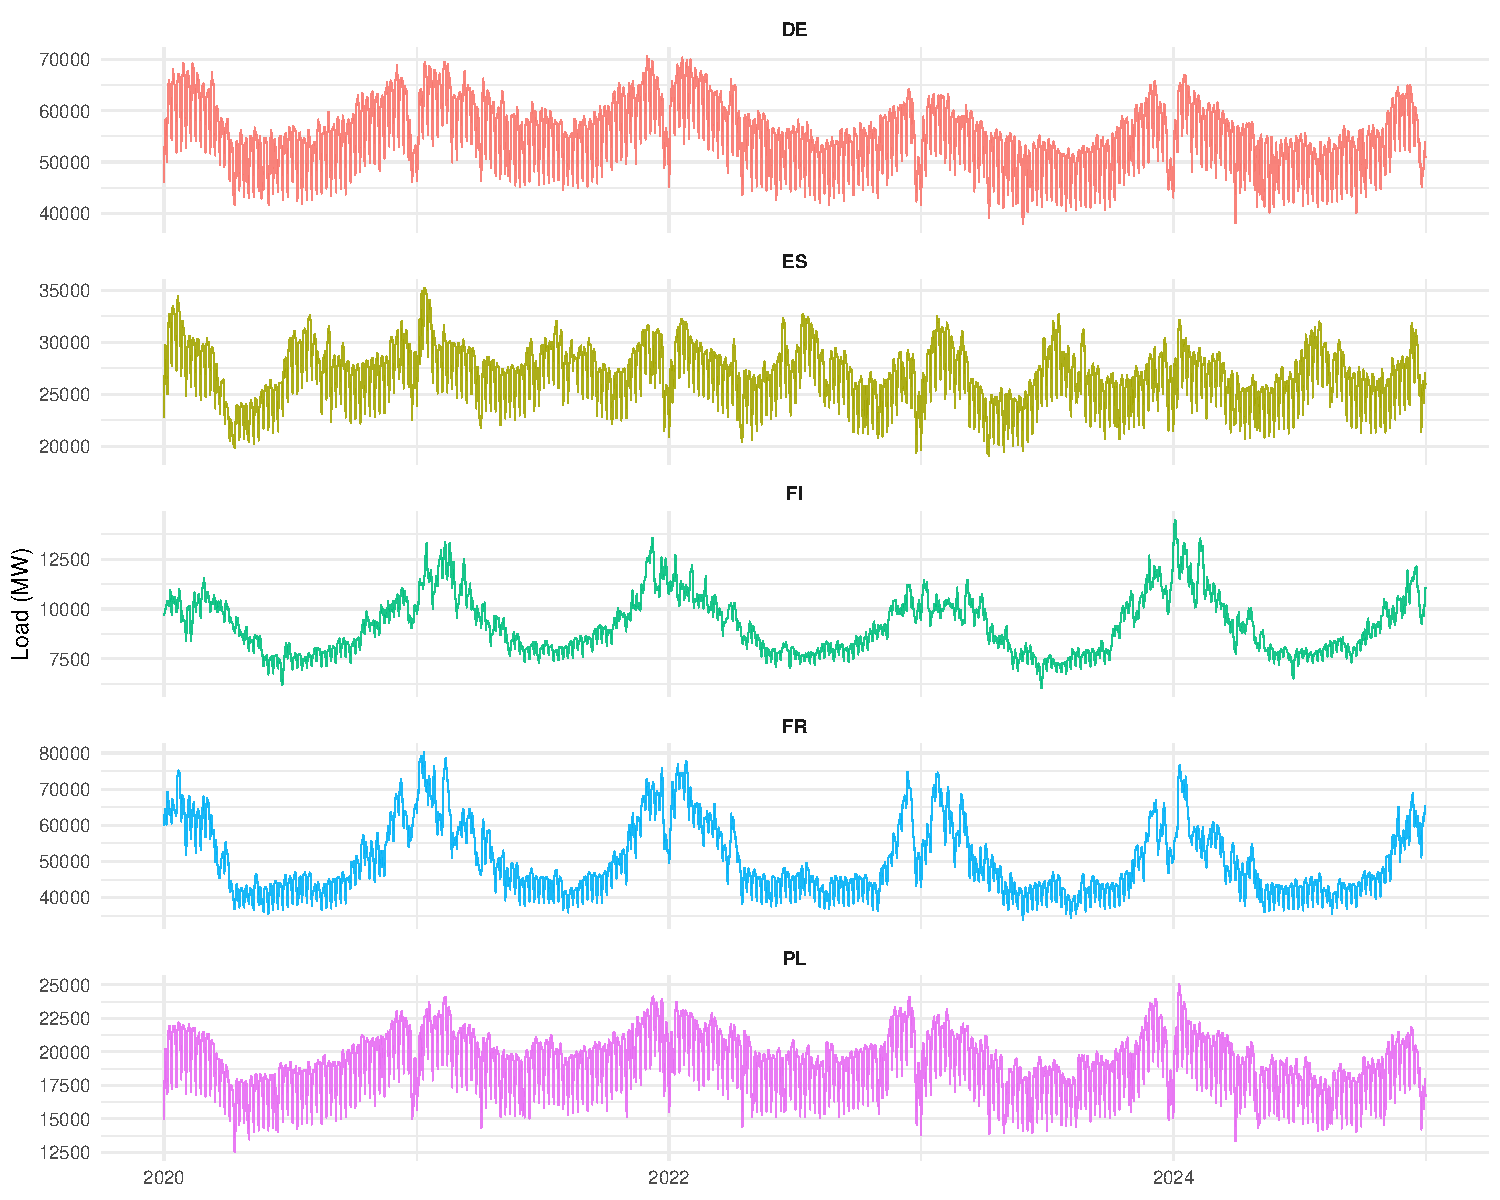
\includegraphics[width=\textwidth]{figures/fig01_load_series.pdf}
  \caption{Daily electricity load, focus countries, 2020-2024.}
  \label{fig:load_series}
\end{figure}

\begin{figure}[H]
  \centering
  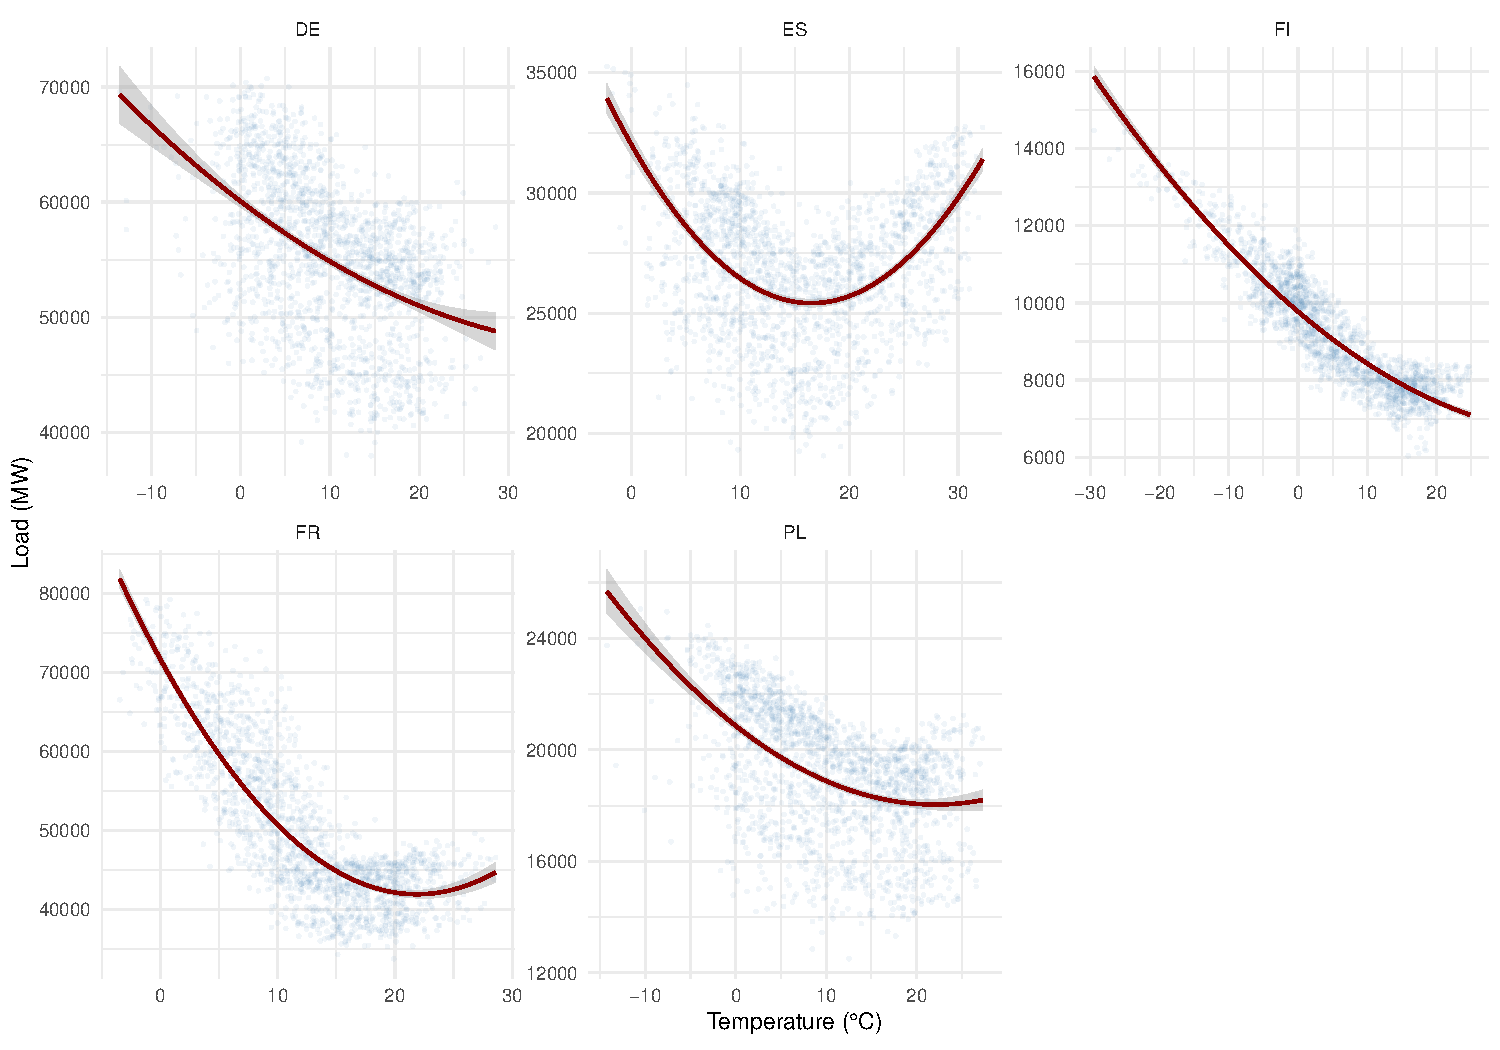
\includegraphics[width=\textwidth]{figures/fig02_temp_load_scatter.pdf}
  \caption{Temperature vs.\ daily load with quadratic fit.}
  \label{fig:scatter}
\end{figure}

\section{Method and Model}
\label{sec:method}

\subsection{Stationarity testing}
\label{sec:stationarity}

Before estimating dynamic models, we test the order of integration of $\ln(L_t)$ and $T_t$ using three complementary tests. A series is declared \textbf{stationary} only when all three agree at the 5\% level.

\paragraph{Augmented Dickey-Fuller (ADF).} The ADF regression augments a random walk with lagged differences:
$\Delta y_t = \alpha + \beta t + \gamma y_{t-1} + \sum_{j=1}^{p}\delta_j \Delta y_{t-j} + u_t$.
$H_0\!: \gamma=0$ (unit root). We select $p$ by the minimum Breusch-Godfrey $p$-value among augmentation orders \citep{pesaran1997}. Rejecting $H_0$ supports stationarity.

\paragraph{Phillips-Perron (PP).} PP tests the same null as ADF but corrects the $t$-statistic for serial correlation and heteroskedasticity in $u_t$. Rejection of the unit-root null supports stationarity.

\paragraph{KPSS.} The KPSS test reverses the null: $H_0$ is stationarity around a constant. The 5\% critical value is $0.46$ \citep{kwiatkowski1992}; a KPSS statistic above $0.46$ rejects stationarity. Non-rejection supports stationarity.

\noindent Table~\ref{tab:stationarity} reports four series per focus country. For $\ln(L_t)$ in levels we test whether log load has a unit root (expected non-stationary for DE, ES, FR, PL). For $\Delta\ln(L_t)$ we test stationarity after differencing (expected stationary, classifying log load as I(1)). For $T_t$ in levels we test whether temperature is I(0) (expected stationary). For $\Delta T_t$ we confirm that differenced temperature remains stationary. For Germany, $\ln(L_t)$ in levels yields ADF $p=0.01$ and PP $p=0.01$, but KPSS $=2.92>0.46$, so the combined verdict is \textbf{non-stationary}. After first-differencing, all three tests classify $\Delta\ln(L_t)$ as stationary (KPSS $=0.007$). The same pattern holds for Spain, France, and Poland; Finland is borderline in levels (KPSS does not reject). Temperature in levels is stationary for all focus countries; first differences remain stationary. We therefore estimate the ARDL in first differences of log load with $\Delta T$ as the weather regressor.

\begin{table}[H]
  \centering
  \caption{Unit-root tests: focus countries (four series per country)}
  \label{tab:stationarity}
  \scriptsize
  
\begin{tabular}{llrlrlrl}
\toprule
Cty & Series & ADF stat & ADF $p$ & PP stat & PP $p$ & KPSS stat & Stationary?\\
\midrule
DE & $\ln(L_t)$ & -19.42 & $0.01$ & -19.81 & $0.01$ & 2.92 & No\\
DE & $\Delta\ln(L_t)$ & -40.77 & $0.01$ & -49.59 & $0.01$ & 0.01 & Yes\\
DE & $T_t$ & -4.65 & $0.01$ & -5.92 & $0.01$ & 0.38 & Yes\\
DE & $\Delta T_t$ & -25.82 & $0.01$ & -38.14 & $0.01$ & 0.03 & Yes\\
ES & $\ln(L_t)$ & -18.30 & $0.01$ & -18.68 & $0.01$ & 1.40 & No\\
ES & $\Delta\ln(L_t)$ & -41.21 & $0.01$ & -49.51 & $0.01$ & 0.01 & Yes\\
ES & $T_t$ & -3.25 & 0.02 & -3.92 & $0.01$ & 0.28 & Yes\\
ES & $\Delta T_t$ & -25.99 & $0.01$ & -38.53 & $0.01$ & 0.07 & Yes\\
FI & $\ln(L_t)$ & -5.84 & $0.01$ & -4.66 & $0.01$ & 0.27 & Yes$^\dag$\\
FI & $\Delta\ln(L_t)$ & -40.84 & $0.01$ & -43.27 & $0.01$ & 0.03 & Yes\\
FI & $T_t$ & -5.03 & $0.01$ & -4.96 & $0.01$ & 0.21 & Yes\\
FI & $\Delta T_t$ & -22.86 & $0.01$ & -38.64 & $0.01$ & 0.02 & Yes\\
FR & $\ln(L_t)$ & -7.85 & $0.01$ & -6.50 & $0.01$ & 0.83 & No\\
FR & $\Delta\ln(L_t)$ & -38.18 & $0.01$ & -40.85 & $0.01$ & 0.03 & Yes\\
FR & $T_t$ & -4.92 & $0.01$ & -6.42 & $0.01$ & 0.24 & Yes\\
FR & $\Delta T_t$ & -25.79 & $0.01$ & -37.85 & $0.01$ & 0.03 & Yes\\
PL & $\ln(L_t)$ & -20.61 & $0.01$ & -21.29 & $0.01$ & 1.08 & No\\
PL & $\Delta\ln(L_t)$ & -43.99 & $0.01$ & -55.80 & $0.01$ & 0.01 & Yes\\
PL & $T_t$ & -4.17 & $0.01$ & -5.18 & $0.01$ & 0.43 & Yes\\
PL & $\Delta T_t$ & -26.01 & $0.01$ & -40.44 & $0.01$ & 0.03 & Yes\\
\bottomrule
\end{tabular}

  \\[0.5em]
  \footnotesize $^\dag$Finland: KPSS does not reject stationarity in levels; we nonetheless model $\Delta\ln(L)$ for consistency across countries.
\end{table}

\subsection{Residual diagnostics: definitions and decision rules}
\label{sec:residual-diagnostics}

Before interpreting static OLS coefficients, we apply a standard post-estimation diagnostic suite. Each test targets a distinct failure mode; rejection at the 5\% level guides the move to dynamic models and HAC inference.

\paragraph{Breusch-Godfrey (BG).} Tests $H_0$: no residual autocorrelation up to order $p$. We report $p$-values at orders 1, 5, 7, and 14 (approximately one day, one work week, one calendar week, and two weeks). Rejection invalidates conventional OLS standard errors and motivates ARDL lags; order~7 rejection specifically motivates the seasonal lag-7 terms in the final specification.

\paragraph{Breusch-Pagan (BP).} Tests $H_0$: homoscedasticity. Rejection indicates heteroskedasticity and motivates HAC-robust standard errors in the ARDL stage.

\paragraph{White.} A more general heteroskedasticity test using an auxiliary regression of squared residuals on fitted values and their squares. Applied to the final seasonal ARDL; rejection confirms that HAC inference remains necessary.

\paragraph{Ramsey RESET.} Tests $H_0$: the linear functional form is adequate. Rejection signals neglected nonlinearity or dynamics not captured by the current regressor set.

\paragraph{Jarque-Bera (JB).} Tests $H_0$: normally distributed residuals. Rejection means exact $t$-tests are inappropriate; inference relies on the large-sample central limit theorem.

\paragraph{Variance inflation factor (VIF).} Measures collinearity among regressors; values above 10 are a common concern. $T_t$ and $T_t^2$ are mechanically correlated; we therefore centre temperature in the supplementary GAM specification.

\subsection{General static OLS specification}
\label{sec:ols-general}

Before estimating dynamic models, we specify a general static OLS in \textbf{levels} for each focus country. Protected regressors are $T_t$, $T_t^2$, month dummies, and a weekend indicator; candidate weather controls are dew point, wind speed, solar radiation, cloud cover, and precipitation:
\begin{equation}
  L_t = \beta_0 + \beta_1 T_t + \beta_2 T_t^2
        + \mathbf{z}_t'\boldsymbol{\alpha}
        + \sum_m \theta_m M_{m,t}
        + \delta\,\mathit{Weekend}_t
        + \varepsilon_t,
  \label{eq:ols_general}
\end{equation}
where $\mathbf{z}_t = (\mathit{DP}_t,\, W_t,\, S_t,\, \mathit{TCC}_t,\, P_t)'$.
Temperature is mean-centred ($\tilde{T}_t = T_t - \bar{T}$) in the VIF robustness check to reduce mechanical collinearity with $T_t^2$.

\subsection{General-to-specific variable selection: static OLS stage}
\label{sec:gts}

We reduce \eqref{eq:ols_general} country by country using nested $F$-tests at the 5\% level: jointly insignificant weather controls are dropped; collinear pairs (notably dew point and solar radiation) are removed when joint tests fail to reject; insignificant month dummies are merged into the January baseline where appropriate. The surviving regressors enter the dynamic ARDL stage in first differences. Table~\ref{tab:gts_de} traces the reduction for Germany; Table~\ref{tab:gts_all} summarises retained controls for all focus countries.

\begin{table}[H]
  \centering
  \caption{General-to-specific OLS reduction --- Germany}
  \label{tab:gts_de}
  \small
  
\begin{tabular}{rllrl}
\toprule
Step & Model & Change & $R^2$ & F-test $p$\\
\midrule
1 & General OLS & Full model with all weather controls & 0.729 & ---\\
2 & Collinearity check (dewpoint, solar) & Test H0: dewpoint_c = solar_radiation_wm2 = 0 & 0.729 & 0.483\\
3 & Joint F on insignificant set & Test H0: dewpoint, solar, month02, month11, precipitation = 0 & 0.729 & 0.030\\
4 & Merge Nov into Jan & month_reduced with Nov merged to Jan baseline & 0.729 & 0.433\\
5 & Drop precipitation (final) & Drop precipitation_mm -> final parsimonious OLS & 0.728 & 0.262\\
\bottomrule
\end{tabular}

  \\[0.5em]
  \footnotesize Retained regressors: $T_t$, $T_t^2$, wind speed, cloud cover,
  reduced month dummies, weekend indicator.
\end{table}

\begin{table}[H]
  \centering
  \caption{Surviving weather controls by country after GTS reduction}
  \label{tab:gts_all}
  \small
  
\begin{tabular}{llllll}
\toprule
Variable & DE & ES & FI & FR & PL\\
\midrule
Dew point ($\mathit{DP}_t$) & $\times$ & $\times$ & $\times$ & \checkmark & \checkmark\\
Wind speed ($W_t$) & \checkmark & \checkmark & \checkmark & $\times$ & $\times$\\
Solar radiation ($S_t$) & $\times$ & $\times$ & $\times$ & \checkmark & $\times$\\
Cloud cover ($\mathit{TCC}_t$) & \checkmark & \checkmark & $\times$ & $\times$ & $\times$\\
Precipitation ($P_t$) & $\times$ & \checkmark & $\times$ & $\times$ & $\times$\\
\textit{Month merges} & \textit{Nov} & \textit{Feb, Jul} & \textit{Dec} & \textit{---} & \textit{Mar, Oct, Nov}\\
\bottomrule
\end{tabular}

  \\[0.5em]
  \footnotesize $\checkmark$ = retained; $\times$ = dropped. Month merges collapse listed months into the January baseline.
\end{table}

\paragraph{VIF check.}
Re-estimating the final OLS with mean-centred temperature ($\tilde{T}_t$), VIF values for all retained regressors fall below 5, confirming that multicollinearity is not a concern in the centred specification.\footnote{VIF values are reported in the replication notebook (\texttt{combined-analysis.Rmd}, Section~5).}

\paragraph{GAM comparison.}
As a nonlinearity check, we estimate a Generalized Additive Model replacing the quadratic temperature term with a penalised cubic regression spline ($k=12$, REML smoothing) while holding the GTS control set fixed. The GAM achieves a lower AIC than the quadratic OLS (Table~\ref{tab:gam_aic}), confirming structure beyond a symmetric parabola. We retain the quadratic form for the dynamic stage and treat the GAM as a diagnostic.

\begin{table}[H]
  \centering
  \caption{AIC comparison: quadratic OLS vs.\ GAM (Germany, static stage)}
  \label{tab:gam_aic}
  \small
  
\begin{tabular}{llr}
\toprule
Model & AIC & $R^2$\\
\midrule
Quadratic OLS (final, centred) & 35,052 & 0.728\\
GAM (spline on T, same controls) & 34,993 & 0.736\\
\bottomrule
\end{tabular}

\end{table}

\subsection{Baseline static OLS for U-curve visualisation}
\label{sec:baseline-ols}

For turning-point estimation and exploratory diagnostics we also estimate a pooled baseline in levels with weekday and month dummies and the full weather set:
\begin{equation}
  L_t = \beta_0 + \beta_1 T_t + \beta_2 T_t^2 + \sum_d \delta_d D_{d,t} + \sum_m \theta_m M_{m,t} + \mathbf{X}_t'\boldsymbol{\gamma} + \varepsilon_t,
  \label{eq:ols}
\end{equation}
where $D_{d,t}$ are weekday dummies, $M_{m,t}$ month dummies, and $\mathbf{X}_t$ additional weather controls. A U-shape requires $\beta_1 < 0$ and $\beta_2 > 0$; the turning point is $T^* = -\beta_1 / (2\beta_2)$. Diagnostic results for \eqref{eq:ols} are in Tables~\ref{tab:baseline_diag} and~\ref{tab:baseline_ols}; BG(7) rejects for every focus country, motivating the dynamic specification below.

\begin{table}[H]
  \centering
  \caption{Baseline OLS diagnostic tests (focus countries)}
  \label{tab:baseline_diag}
  \small
  
\begin{tabular}{llllrr}
\toprule
Country & BP $p$ & RESET $p$ & JB $p$ & BG(1) $p$ & BG(7) $p$\\
\midrule
DE & $\approx 0$ & 0.046 & $\approx 0$ & 0 & 0\\
ES & $\approx 0$ & 0.314 & $\approx 0$ & 0 & 0\\
FI & $\approx 0$ & $\approx 0$ & $\approx 0$ & 0 & 0\\
FR & $\approx 0$ & $\approx 0$ & $\approx 0$ & 0 & 0\\
PL & $\approx 0$ & 0.013 & $\approx 0$ & 0 & 0\\
\bottomrule
\end{tabular}

\end{table}

\subsection{General-to-specific model selection: dynamic ARDL stage}
\label{sec:gts_ardl}

Having fixed the weather control set from the static GTS stage (Table~\ref{tab:gts_all}), we build up to the seasonal ARDL in nested steps on daily data in first differences. For Germany, $\Delta W_t$ and $\Delta\mathit{TCC}_t$ enter alongside temperature lags; other countries use their country-specific retained controls in first differences. The reduction path for Germany is in Table~\ref{tab:gts_ardl_de}.

\begin{itemize}
  \item \textbf{DL full $\to$ DL parsimonious:} drop $L(\Delta T_t, 2)$ (insignificant; AIC improves from $-6546.3$ to $-6548.2$). Country-specific $\Delta W_t$, $\Delta\mathit{TCC}_t$, etc.\ are retained.
  \item \textbf{DL parsimonious $\to$ ARDL full:} add $L(\Delta\ln L_t, 1{:}2)$. BG(1) improves from $\approx 0$ to $0.041$.
  \item \textbf{ARDL full $\to$ ARDL parsimonious:} drop $L(\Delta T_t, 2)$ again (still insignificant).
  \item \textbf{ARDL parsimonious $\to$ Seasonal ARDL (final):} add $L(\Delta\ln L_t, 7)$ and $L(\Delta T_t, 7)$ to absorb the lag-7 ACF spike (Figure~\ref{fig:ols_acf}).
\end{itemize}

\begin{table}[H]
  \centering
  \caption{General-to-specific ARDL reduction --- Germany}
  \label{tab:gts_ardl_de}
  \small
  
\begin{tabular}{lrlll}
\toprule
Model step & AIC & BG(1) $p$ & BG(7) $p$ & SR temp sum\\
\midrule
DL full & -6546.3 & $\approx 0$ & $\approx 0$ & -0.0068\\
DL parsimonious & -6548.2 & $\approx 0$ & $\approx 0$ & -0.0070\\
ARDL full & -6699.1 & 0.041 & $\approx 0$ & -0.0072\\
ARDL parsimonious & -6700.7 & 0.037 & $\approx 0$ & -0.0070\\
Seasonal ARDL (final) & -6683.1 & 0.031 & $\approx 0$ & -0.0073\\
\bottomrule
\end{tabular}

\end{table}

\subsection{Main model: seasonal ARDL}
\label{sec:ardl}

Following \citet{pesaran1997}, the preferred seasonal specification is:
\begin{equation}
  \Delta \ln(L_t) = \sum_{i \in \{1,2,7\}} \phi_i \Delta \ln(L_{t-i})
  + \sum_{j \in \{0,1,3,7\}} \beta_j \Delta T_{t-j}
  + \gamma \Delta T_t^2
  + \boldsymbol{\kappa}'\Delta\mathbf{z}_t
  + \sum_d \delta_d D_{d,t}
  + u_t,
  \label{eq:ardl}
\end{equation}
where $D_{d,t}$ are weekday fixed effects, lag~7 captures weekly seasonality, and $\Delta\mathbf{z}_t$ contains the country-specific first-differenced weather controls retained in Table~\ref{tab:gts_all} (e.g.\ $\Delta W_t$ and $\Delta\mathit{TCC}_t$ for Germany; $\Delta\mathit{DP}_t$ and $\Delta S_t$ for France). Parsimony is assessed via ANOVA where sample sizes match; otherwise AIC and BG(7) are compared.

\paragraph{Parameter interpretation.}
The \textbf{short-run temperature effect} is $\sum_j \hat{\beta}_j$ (contemporaneous and lagged $\Delta T$ coefficients only, excluding $\Delta T^2$). Because we estimate in first differences of log load, this sum approximates the cumulative elasticity of daily load with respect to a one-degree sustained change in temperature over the distributed lag window.

\noindent Individual lag coefficients carry distinct economic meaning. The contemporaneous term $\hat{\beta}_0$ captures same-day load adjustment; $\hat{\beta}_1$ reflects next-day persistence; $\hat{\beta}_3$ likely picks up weekly work patterns or slow building thermal mass; $\hat{\beta}_7$ captures weekly seasonal co-movement between temperature and load. The sum $\sum_j \hat{\beta}_j$ aggregates these channels into a single short-run multiplier comparable across countries.

\noindent A \textbf{long-run} temperature multiplier would require a levels ARDL or error-correction representation; we leave this to future work and note that the short-run sum is the appropriate interpretable quantity in the differenced specification.

\subsection{Post-estimation diagnostics on the final ARDL}
\label{sec:ardl-diagnostics}

On the selected seasonal ARDL we report Breusch-Pagan and White tests for homoscedasticity, Ramsey RESET for neglected nonlinearity, and Breusch-Godfrey at orders 1, 5, 7, and 14. Results appear in Table~\ref{tab:ardl_diag}. Rejection of BP or White motivates HAC-robust standard errors \footnote{Inference utilizes Newey-West HAC robust standard errors via the \texttt{sandwich::vcovHAC} package.}; persistent BG(7) rejection is acknowledged as a limitation.

\subsection{Comparison designs}

We compare the final seasonal ARDL with a daily \texttt{auto.arima} model on the same $\Delta\ln(L_t)$ sample (weather and weekday \texttt{xreg}, lag-7 alignment) using AIC and BIC. Separately, for German hourly load we hold out the last 14 days and compare a seasonal ARIMA with temperature and hour-of-day controls against a seasonal-naive benchmark (period 24). Full comparison results are in Section~\ref{sec:results}.

\section{Results}
\label{sec:results}

\subsection{Baseline OLS and U-curve}
\label{sec:baseline-results}

Table~\ref{tab:baseline_ols} reports U-curve coefficients and turning points. Country-specific turning points have a clear climate interpretation: DE switches from heating to cooling demand at $17.9\,^\circ$C, ES at $15.9\,^\circ$C, FI at $20.7\,^\circ$C, FR at $17.8\,^\circ$C, and PL at $21.1\,^\circ$C (Figure~\ref{fig:turning_points}).

\noindent BG(1) and BG(7) reject for all five countries ($p \approx 0$), indicating autocorrelation that weekday dummies do not absorb (Figure~\ref{fig:ols_acf}). Combined with BP, RESET, and JB rejections (Table~\ref{tab:baseline_diag}), static OLS is not an appropriate inferential model; we proceed to the GTS ARDL results below.

\begin{figure}[H]
  \centering
  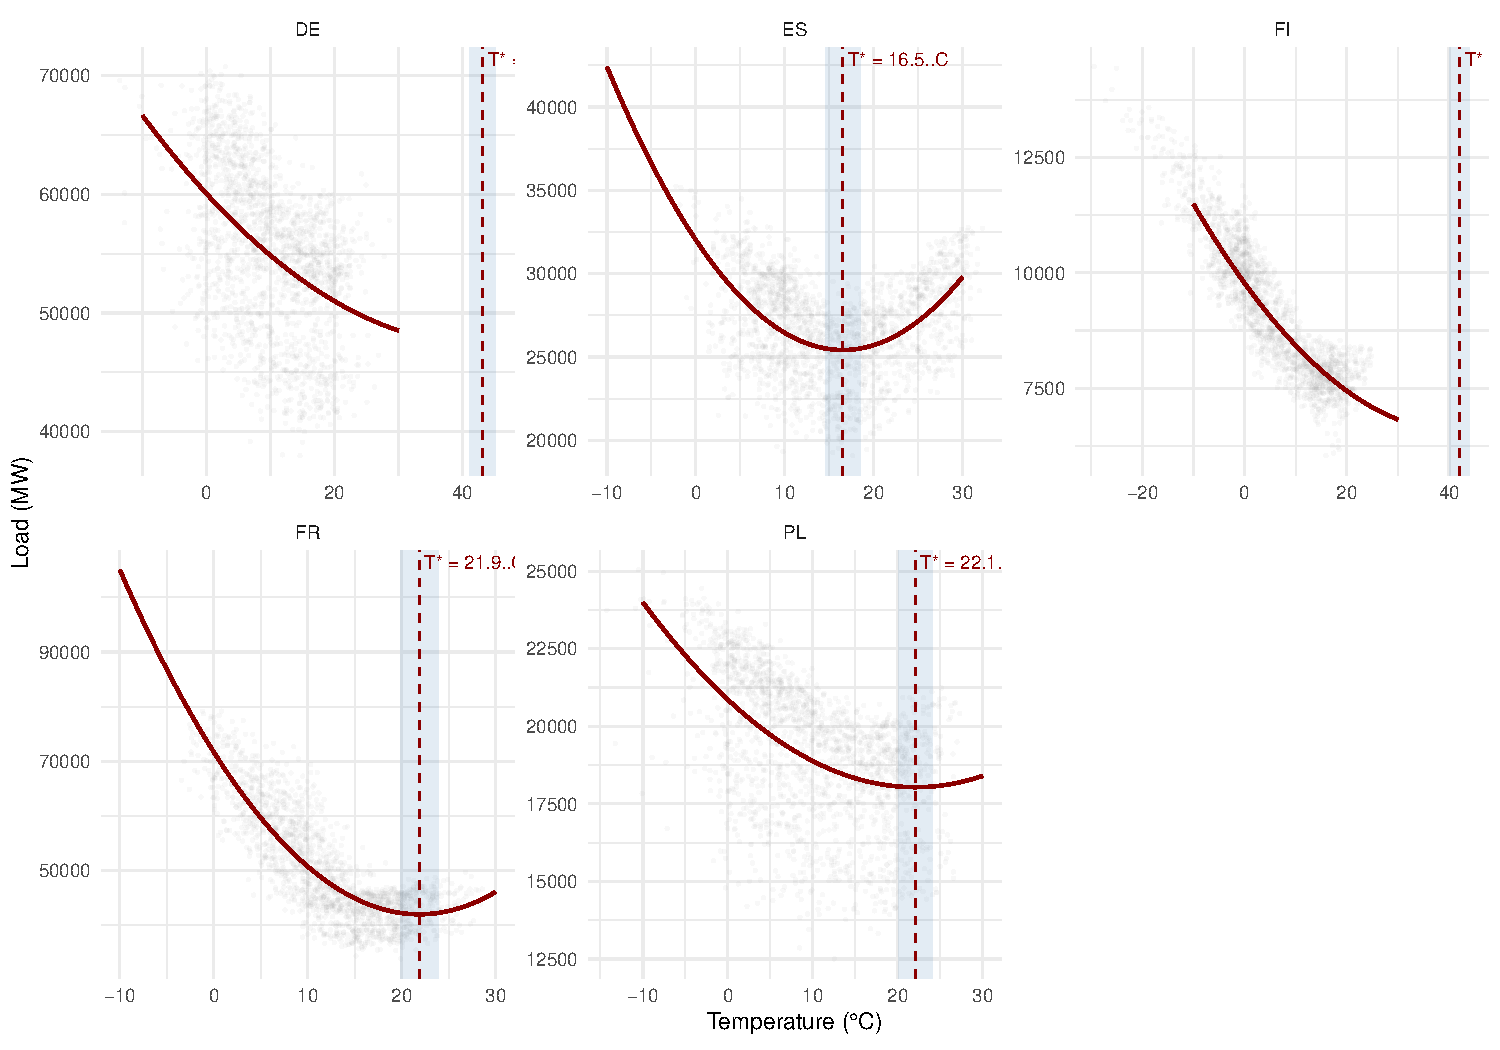
\includegraphics[width=\textwidth]{figures/fig06_turning_points.pdf}
  \caption{Country-specific U-curve fits with turning point ($T^*$, dashed) and comfort zone ($T^* \pm 2\,^\circ$C, shaded band).}
  \label{fig:turning_points}
\end{figure}

\begin{table}[H]
  \centering
  \caption{Baseline OLS: U-curve and residual diagnostics (focus countries)}
  \label{tab:baseline_ols}
  \small
  
\begin{tabular}{lrlrrll}
\toprule
Country & $R^2$ & $\hat{\beta}_1$ & $\hat{\beta}_2$ & Turning pt ($^\circ$C) & BG(7) $p$ & RESET $p$\\
\midrule
DE & 0.729 & -512 & 13.9 & 18.5 & $\approx 0$ & 0.046\\
ES & 0.713 & -585 & 18.3 & 15.9 & $\approx 0$ & 0.314\\
FI & 0.916 & -104 & 2.6 & 20.4 & $\approx 0$ & $\approx 0$\\
FR & 0.899 & -1,864 & 52.6 & 17.7 & $\approx 0$ & $\approx 0$\\
PL & 0.701 & -321 & 7.5 & 21.3 & $\approx 0$ & 0.013\\
\bottomrule
\end{tabular}
 
\end{table}

\begin{figure}[H]
  \centering
  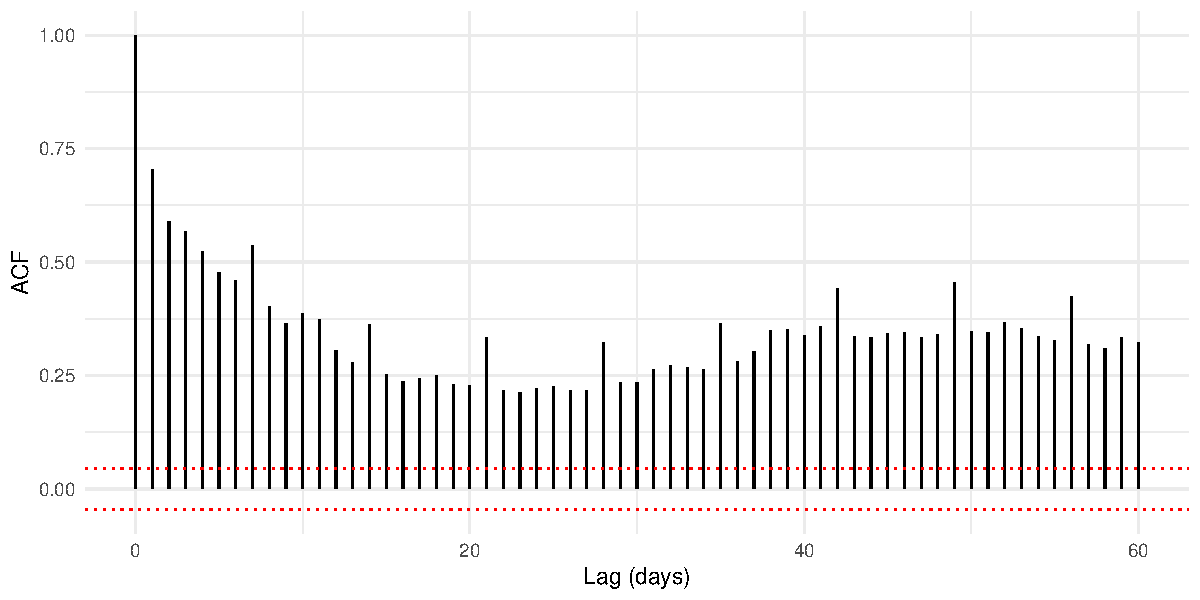
\includegraphics[width=0.85\textwidth]{figures/fig03_ols_acf_de.pdf}
  \caption{Baseline OLS residual ACF, Germany.}
  \label{fig:ols_acf}
\end{figure}

\subsection{Seasonal ARDL results}
\label{sec:ardl-results}

Table~\ref{tab:ardl} reports the seasonal ARDL summary for focus countries (HAC-robust standard errors where Table~\ref{tab:ardl_diag} indicates heteroskedasticity or residual autocorrelation). Figure~\ref{fig:ardl_acf} shows reduced lag-1 autocorrelation relative to OLS for Germany.

\begin{table}[H]
  \centering
  \caption{Final seasonal ARDL diagnostic tests - focus countries}
  \label{tab:ardl_diag}
  \small
  
\begin{tabular}{llllll}
\toprule
Country & BP $p$ & White $p$ & RESET $p$ & BG(1) $p$ & BG(7) $p$\\
\midrule
DE & $\approx 0$ & $2.5\times 10^{-5}$ & 0.572 & 0.031 & $\approx 0$\\
ES & $\approx 0$ & $<0.01$ & 0.625 & $<0.01$ & $\approx 0$\\
FI & 0.081 & 0.042 & $\approx 0$ & 0.088 & $\approx 0$\\
FR & $\approx 0$ & $9.7\times 10^{-6}$ & 0.968 & $\approx 0$ & $\approx 0$\\
PL & $\approx 0$ & $2.2\times 10^{-6}$ & 0.014 & 0.104 & $\approx 0$\\
\bottomrule
\end{tabular}

\end{table}

\begin{table}[H]
  \centering
  \caption{Seasonal ARDL: short-run temperature effect and BG diagnostics}
  \label{tab:ardl}
  
\begin{tabular}{lllll}
\toprule
Country & Short-run $\sum \hat{\beta}_j$ & BG(1) $p$ & BG(7) $p$ & AIC\\
\midrule
DE & -0.0073 & 0.031 & $\approx 0$ & -6,683\\
ES & -0.0087 & $<0.01$ & $\approx 0$ & -7,144\\
FI & -0.0093 & 0.088 & $\approx 0$ & -8,798\\
FR & -0.0197 & $\approx 0$ & $\approx 0$ & -7,641\\
PL & -0.0113 & 0.104 & $\approx 0$ & -6,294\\
\bottomrule
\end{tabular}

\end{table}

\begin{figure}[H]
  \centering
  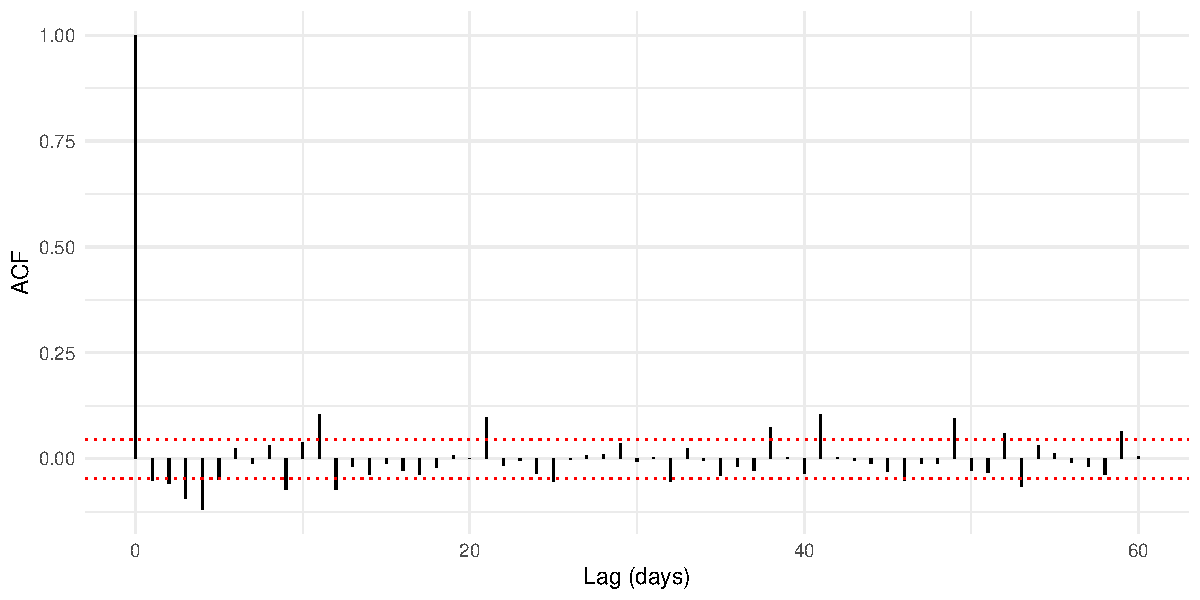
\includegraphics[width=0.85\textwidth]{figures/fig04_ardl_acf_de.pdf}
  \caption{Seasonal ARDL residual ACF, Germany.}
  \label{fig:ardl_acf}
\end{figure}

\noindent Persistent BG(7) rejection reflects weekly load seasonality from holidays, shift-work cycles, and school calendars that a single lag-7 term cannot fully absorb. Extensions include lag-14 terms, temperature-interacted weekday dummies, or hourly estimation with explicit hour-of-day effects (Section~\ref{sec:forecast-results}). All coefficient inference uses HAC-robust standard errors \footnote{Inference utilizes Newey-West HAC robust standard errors via the \texttt{sandwich::vcovHAC} package.}.

\subsection{ARDL vs.\ ARIMA (daily Germany)}
\label{sec:ardl-arima-results}

Table~\ref{tab:ardl_arima} compares the final seasonal ARDL with \texttt{auto.arima} on the same daily $\Delta\ln(L)$ sample. The seasonal ARDL achieves a lower AIC ($-6683$ vs.\ $-6621$) and lower BIC on the aligned sample, while also yielding interpretable short-run elasticities.

\noindent The ARIMA(1,0,3) alternative remains competitive and trades structural lags for a parsimonious MA polynomial. We retain the seasonal ARDL as the main model because its coefficients answer policy-relevant questions at specific lag horizons (Section~\ref{sec:ardl}) and because each term was retained via the general-to-specific path (Tables~\ref{tab:gts_de} and~\ref{tab:gts_ardl_de}) rather than automatic order selection alone.

\begin{table}[H]
  \centering
  \caption{Daily ARDL vs.\ ARIMA - Germany (same $\Delta\ln(L)$ sample)}
  \label{tab:ardl_arima}
  
\begin{tabular}{lrrl}
\toprule
Model & AIC & BIC & ARIMA order\\
\midrule
Seasonal ARDL (final) & -6683.1 & -6584 & -\\
ARIMA + weather \texttt{xreg} & -6621.0 & -6544 & (1,0,3)\\
\bottomrule
\end{tabular}

\end{table}

\subsection{Hourly forecast robustness (Germany)}
\label{sec:forecast-results}

Table~\ref{tab:forecast} compares the hourly ARIMA + weather model against a seasonal-naive benchmark on the 14-day holdout. The ARIMA model reduces MAE by approximately 40\% and MAPE from 17.8\% to 10.9\%.

\begin{table}[H]
  \centering
  \caption{Out-of-sample forecast accuracy: DE hourly load (14-day holdout, MW levels)}
  \label{tab:forecast}
  
\begin{tabular}{llll}
\toprule
Model & MAE (MW) & RMSE (MW) & MAPE\\
\midrule
ARIMA + weather \texttt{xreg} & 5,328 & 6,823 & 10.9\%\\
Seasonal naive (period 24) & 8,844 & 10,764 & 17.8\%\\
\bottomrule
\end{tabular}

\end{table}

\begin{figure}[H]
  \centering
  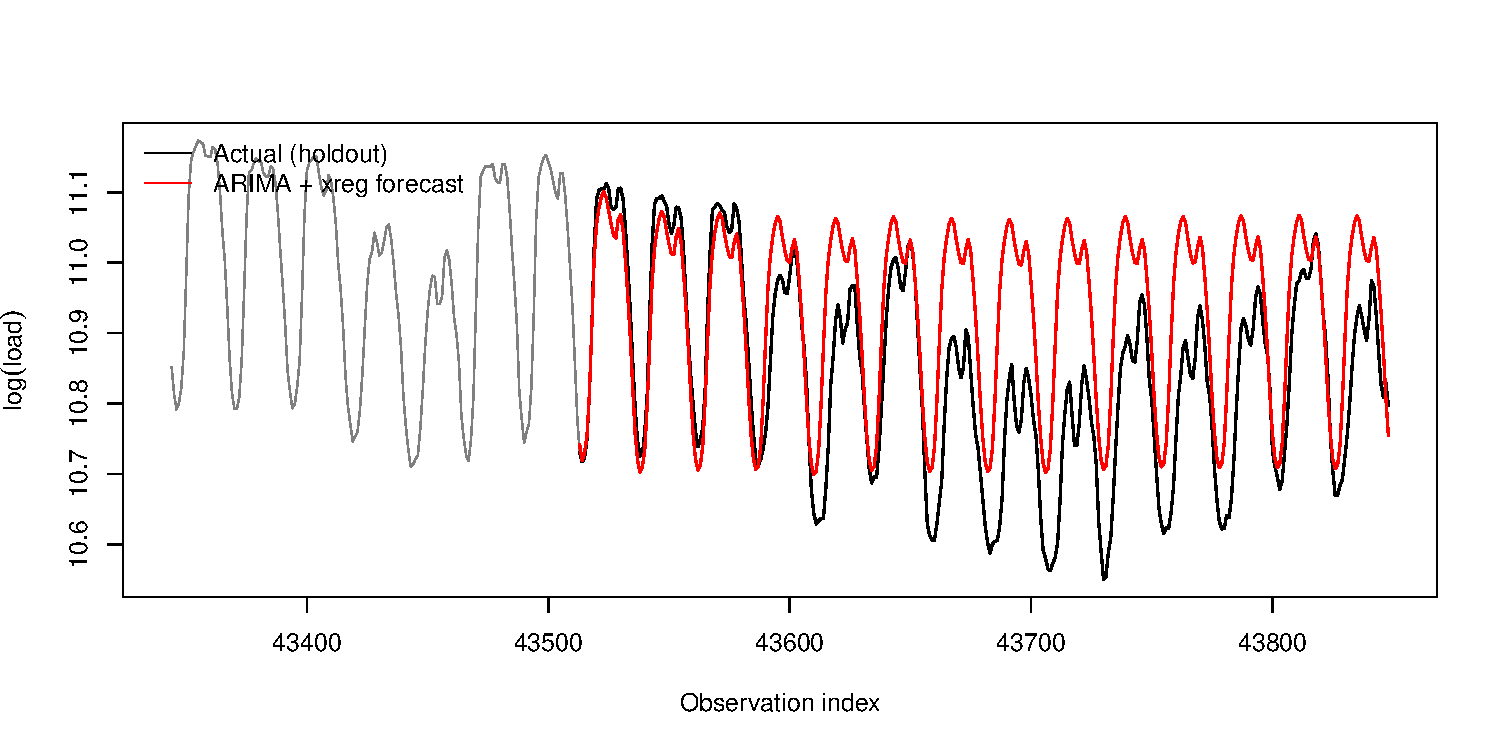
\includegraphics[width=\textwidth]{figures/fig05_de_forecast.pdf}
  \caption{DE hourly log(load): holdout forecast vs.\ actual (last 14 days of sample).}
  \label{fig:forecast}
\end{figure}

\subsection{Hypothesis verification}
\label{sec:hypotheses}

Table~\ref{tab:hypotheses} summarises the verdict on each hypothesis with the econometric reason for partial rejection where applicable.

\begin{table}[H]
  \centering
  \caption{Hypothesis verification summary}
  \label{tab:hypotheses}
  \small
  \begin{tabular}{p{1.2cm}p{3.2cm}p{2.2cm}p{6.5cm}}
    \toprule
    ID & Statement & Verdict & Explanation \\
    \midrule
    H1 & U-shaped temperature-load relationship & Supported & $\hat{\beta}_1 < 0$, $\hat{\beta}_2 > 0$ in \eqref{eq:ols}; $R^2$ 0.74-0.92; turning points 16-21\,$^\circ$C (Table~\ref{tab:baseline_ols}). \\
    H2 & ARDL reduces autocorrelation vs.\ OLS & Partially supported & BG(7) rejects under OLS for all focus countries; seasonal ARDL improves BG(1) for DE ($p = 0.031$) but BG(7) still $\approx 0$ (Table~\ref{tab:ardl}). HAC SEs used for inference. \\
    H3 & Cross-country heterogeneity in short-run temp effects & Partially supported &
Magnitudes differ substantially across focus countries (FR: $-0.020$; FI: $-0.009$;
DE: $-0.007$), consistent with France's large nuclear-heated building stock and Finland's
heating dominance. All short-run sums are negative, including ES ($-0.009$), which is
unexpected under a cooling-dominated hypothesis. The most likely explanation is that daily
load averaging masks intra-day cooling peaks, and Spain's sample mean temperature of $15.5\,^\circ$C keeps the
series in the heating arm of the U-curve for most observations. \\
    H4 & ARIMA + weather beats seasonal naive (hourly DE) & Supported & MAE 5,327 vs.\ 8,844 MW; MAPE 10.9\% vs.\ 17.8\% (Table~\ref{tab:forecast}). \\
    \bottomrule
  \end{tabular}
\end{table}

\section{Findings}
\label{sec:findings}

This paper provides a reproducible analysis of weather-driven electricity demand across 21 European countries. Four main findings emerge.

\noindent First, static OLS confirms a U-shaped temperature-load relationship (\textbf{H1 supported}): comfort temperatures of 16-21\,$^\circ$C across focus countries align with \citet{bessec2008} and \citet{apadula2012}. Second, diagnostic tests reveal strong residual autocorrelation at a weekly lag under OLS; the general-to-specific ARDL path improves first-order autocorrelation for Germany but does not fully eliminate BG(7) rejection (\textbf{H2 partially supported}). We therefore rely on HAC-robust inference for coefficient tests. Third, short-run temperature effects in the final ARDL are negative for all focus countries, with heterogeneity in magnitude (\textbf{H3 partially supported}); Spain's negative sign likely reflects daily aggregation and centroid weather rather than absence of cooling demand. Fourth, both daily and hourly ARIMA specifications with weather controls outperform simpler benchmarks on information criteria or forecast accuracy (\textbf{H4 supported}), consistent with \citet{weron2014}.

\paragraph{Comparison with the literature.}
Turning points in the full 21-country panel (Appendix~\ref{app:full}) fall within ranges reported for European electricity demand. The failure of static OLS diagnostics mirrors the motivation for dynamic models in \citet{pesaran1997}. The forecast gain from weather \texttt{xreg} aligns with the load-forecasting literature.

\paragraph{Limitations and future directions.}
Population-weighted weather reduces but does not eliminate spatial aggregation error; placing the GPW v4 GeoTIFF in the replication pipeline enables full gridded weights (Appendix~\ref{app:replication}). Eight countries were dropped at merge. Persistent BG(7) rejection suggests lag-14 terms or hourly ARDL with explicit day-of-week seasonality. Long-run temperature multipliers could be estimated via a levels ARDL or ECM. Out-of-sample forecast comparison between daily ARDL and ARIMA would strengthen model selection beyond in-sample AIC.

\section*{Data and Code Availability}

Replication code is available on GitHub (\url{https://github.com/giangphuongtran/advanced-econometrics}, release tag \texttt{v1.0}). 
The cleaned daily panel, hourly merged panel, exported tables, and compiled \texttt{report.pdf} are archived at Zenodo: \url{https://doi.org/10.5281/zenodo.20493282}.
Full estimation output, diagnostic tables, and country-by-country GTS paths are available in the \href{../combined-analysis.html}{analysis notebook}. See Appendix~\ref{app:replication} for the full two-tier reproduction workflow.

\bibliographystyle{apalike}
\bibliography{references}

\appendix

\section{Replication pipeline}
\label{app:replication}

Replication artefacts are hosted in two locations: source code on GitHub (\url{https://github.com/giangphuongtran/advanced-econometrics}, release tag \texttt{v1.0}) and the archived merged dataset on Zenodo (\url{https://doi.org/10.5281/zenodo.20493282}). Two reproduction paths are supported.

\subsection*{Fast path (no API keys required)}

\begin{enumerate}
  \item Clone the GitHub repository at tag \texttt{v1.0}.
  \item Download the Zenodo archive and unpack into \texttt{final-project/data/}.
  \item Install dependencies: \texttt{pip install -r requirements.txt} and \texttt{Rscript setup-r.R} (or \texttt{renv::restore()}).
  \item From \texttt{final-project/}: run \texttt{make all}. This regenerates all CSV tables (\texttt{make tables}), figures (\texttt{make figures}), and the compiled \texttt{report.pdf} (\texttt{make report}) from the archived merged panel.
\end{enumerate}

\subsection*{Full path (raw API re-download)}

This path rebuilds the merged daily panel from ENTSO-E and ERA5 sources and requires personal API credentials. It is equivalent to \texttt{make raw-data \&\& make all}.

\begin{enumerate}
  \item \textbf{Population.} \texttt{codes/01\_download\_population.py} fetches Eurostat \texttt{demo\_pjan} totals and builds GPW v4 grid weights (\texttt{gpw\_grid\_weights.parquet}). Place \texttt{gpw\_v4\_population\_2020.tif} from NASA SEDAC in \texttt{data/} for full spatial weighting.
  \item \textbf{ENTSO-E load.} \texttt{codes/02\_download\_load.py} downloads hourly actual load by bidding zone. Requires \texttt{ENTSOE\_API\_KEY} (register at \url{https://transparency.entsoe.eu/}).
  \item \textbf{ERA5 weather.} \texttt{codes/03\_download\_weather.py} retrieves reanalysis from the Copernicus Climate Data Store. Requires a CDS token in \texttt{\textasciitilde/.cdsapirc}.
  \item \textbf{Merge.} \texttt{codes/04\_merge\_data.py} harmonises ERA5 streams, applies population-weighted weather aggregation, and joins to hourly load $\rightarrow$ \texttt{final\_integrated\_u\_curve\_dataset.parquet}.
  \item \textbf{Daily panel.} \texttt{codes/05\_build\_daily\_panel.py} aggregates hourly to daily $\rightarrow$ \texttt{daily\_integrated\_u\_curve\_dataset.parquet}.
  \item Run the fast path from step~3 onwards.
\end{enumerate}

Optional targets: \texttt{make analysis} knits \texttt{combined-analysis.Rmd}; \texttt{make clean} removes derived CSV and PDF artefacts while preserving source data in \texttt{data/}.

\section{Full 21-country summary}
\label{app:full}

Table~\ref{tab:appendix} reports OLS $R^2$, U-curve turning points, seasonal ARDL short-run temperature sums, and BG(1) $p$-values for all countries in the panel.

\begin{table}[H]
  \centering
  \caption{All-country summary (seasonal ARDL and baseline OLS)}
  \label{tab:appendix}
  \scriptsize
  
\begin{tabular}{llllll}
\toprule
Country & Mean $T$ ($^\circ$C) & OLS $R^2$ & Turning pt & SR temp sum & BG(1) $p$\\
\midrule
AT & 5.8 & 0.776 & 13.2 & -0.0078 & 0.136\\
BE & 11.2 & 0.774 & 16.8 & -0.0096 & $<0.01$\\
BG & 11.6 & 0.892 & 14.9 & -0.0152 & 0.025\\
CZ & 9.7 & 0.812 & 20.3 & -0.0127 & 0.073\\
DE & 9.9 & 0.729 & 18.5 & -0.0073 & 0.031\\
DK & 9.1 & 0.788 & 16.1 & -0.0053 & 0.092\\
ES & 15.5 & 0.713 & 15.9 & -0.0087 & $<0.01$\\
FI & 5.2 & 0.916 & 20.4 & -0.0093 & 0.088\\
FR & 12.3 & 0.899 & 17.7 & -0.0197 & $\approx 0$\\
GR & 13.9 & 0.822 & 11.7 & -0.0187 & $<0.01$\\
HR & 10.9 & 0.728 & 11.1 & -0.0099 & $\approx 0$\\
HU & 12.5 & 0.750 & 14.4 & -0.0091 & 0.013\\
IE & 10.5 & 0.643 & 18.6 & -0.0108 & $<0.01$\\
IT & 17.4 & 0.686 & 16.5 & -0.0195 & 0.143\\
NL & 11.5 & 0.739 & 18.7 & -0.0016 & 0.066\\
PL & 10.3 & 0.701 & 21.3 & -0.0113 & 0.104\\
PT & 17.2 & 0.761 & 18.3 & -0.0102 & 0.068\\
RO & 10.7 & 0.646 & 18.4 & -0.0063 & 0.043\\
SE & 7.5 & 0.930 & 20.0 & -0.0110 & 0.115\\
SI & 11.8 & 0.671 & 14.6 & -0.0107 & 0.081\\
SK & 9.5 & 0.622 & 20.5 & -0.0095 & 0.074\\
\bottomrule
\end{tabular}

\end{table}

\end{document}
